%Preamble
\documentclass[12pt,letter]{article}
\usepackage[utf8]{inputenc}
%Layout/Spacing
\usepackage[left=0.7in,right=0.7in,top=1in,bottom=1in]{geometry} %sets margins
\usepackage{setspace} %singles spacing
\usepackage{authblk} %allows multiple athors and affiliations
%Graphics
\usepackage{graphicx} %for inserting pics
\usepackage{pgfplots} %for simple plots
\usepackage[section]{placeins} %for FloatBarrier
\usepackage[linguistics]{forest} %for forests
\usepackage{tikz}% for flow chart
\usetikzlibrary{shapes,arrows,positioning,fit,shapes.misc}%flow chart
\usepackage{tikz-network}
%Tables
\usepackage{tabularx}
\usepackage{multirow}
\usepackage{array}
%Referenes
\usepackage[natbib=true,
            style=nature,
            backend=biber,
            useprefix=true]{biblatex}
\addbibresource{../refs.bib}
%Misc
\usepackage{amsmath} %for math command
%Abbreviations
\usepackage{acro}
%CRISPR-Cas
\DeclareAcronym{crspc}{
    short = CRISPR-Cas,
    long  = CRISPR associated
}
%cas
\DeclareAcronym{cas}{
    short = Cas,
    long  = CRISPR-associated
}
%crispr
\DeclareAcronym{crsp}{
    short = CRISPR,
    long  = Clustered Regularly Interspaced Short Palindromic Repeat
}
%ctmc-fss
\DeclareAcronym{mc}{
    short = CTMC-FFS,
    long  = Continuous-time Markov chain with finite state space
}
%s areus
\DeclareAcronym{sau}{
    short = \textit{S. aureus},
    long  = \textit{Staphylococcus aureus}
}
%ecoli
\DeclareAcronym{ecoli}{
    short = \textit{E. coli},
    long  = \textit{Escherichia coli}
}
%mge
\DeclareAcronym{mge}{
    short = MGE,
    long  = Mobile Genetic Element
}
%hgt
\DeclareAcronym{hgt}{
    short = HGT,
    long  = Horiznotal Gene Transfer
}
%otu
\DeclareAcronym{otu}{
    short = OTU,
    long  = Operation Taxonomic Unit
}
%pa
\DeclareAcronym{pa}{
    short = P/A,
    long  = Presence/Absence,
}
\begin{document}
%Title
\title{Understanding CRISPR and Horizontal Gene Transfer Rates:\\\vspace{0.2cm}
        A Network Theoretic Approach\\ \vspace{0.5cm}
       \Large MolBiol 4C12 Progress Report}
%Authors
\author[1]{Siddharth Reed\thanks{To whom correspondence should be addressed; reeds4@mcmaster.ca}}
\author[1]{G. Brian Golding\vspace{-0.45cm}}
\affil[1]{Department of Biology, McMaster University, Hamilton, Canada}
%\affil[1]{Department of Biology, McMaster University\authorcr
%                Hamilton, Canada}
\date{\today}
\maketitle
%Abstract
\begin{abstract}
    \ac{hgt} is a mechanism by which organisms (mainly prokaryotes) can share genetic material outside of inheritance.
    \ac{hgt} has proven to have significant effects on bacterial genome evolution, allowing for increased genetic diversity and niche adaptation.
    \ac{crspc} is an adaptive immune system in prokaryotes that has garnered much research attention due to it's application as a gene editing tool.
    While much of the focus on \ac{crspc} systems has been related to this application, \ac{crspc} has been shown to have a highly complex interaction with \ac{hgt}.
    Effort has mostly been focused on how \ac{crspc} systems affect the mechanisms of \ac{hgt} and little is currently known about the effects of \ac{crspc} on \ac{hgt} rate, both for individuals and on a population level.
    Proposed here is a network-theoretic approach to further the understanding of the effects of the presence of \ac{crspc} systems on \ac{hgt} within a population.
    Network theory has already been applied to better model evolution and relatedness among bacteria, accounting for \ac{hgt} which traditional phylogenetic methods ignore.
    This network-theoretic approach allows for study of \ac{crspc} effects on individual bacteria as well as population level effects on \ac{hgt}.
    Understanding the effects of \ac{crspc} on \ac{hgt} may help develop strategies to curb spreading antibiotic resistance, understanding bacterial evolution and extend the functionality of \ac{crspc} gene editing systems.
\end{abstract}
\newpage
\linespread{1.25}%default is 1.2, 1.2*1.25 = 1.5 spacing
%TODO
%add results to abstract
%add phylogenetic network plot
%add pan-genome ecoli plot
%expand methods
%add results
%add discussion
%add significance
%add future work

\section*{CRISPR-Cas Systems}
\subsection*{What Are They?}
\ac{crspc} systems are sets of nucleotide motifs (spacers) interspaced with nucleotide repeats (\ac{crsp}s) and \ac{cas} proteins (usually adjacent to the \ac{crsp} motifs) that have an adaptive immune function in many bacteria and archaea\citep{crispgen}.
Each nucleotide motif is indicative of some DNA sequence that was taken up previously by the host and serves as a marker for the \ac{cas} proteins to degrade any foreign DNA matching this motif\citep{crispgen}.
If a bacterium which possesses a \ac{crspc} system is infected with a phage and survives, a motif representative of that phage can be integrated into the \ac{crsp} repeats so that when the ,bacterium is reinfected with the same phage strain it will be detected and degraded by a \ac{cas} protein before genomic integration can occur.
\ac{crsp} is an adaptive immune system, as the bacterium acquire resistance after an unsuccessful infection through spacer integration.\par
Although \ac{crspc} is primarily considered an immune system, non-viral spacers representative of bacterial \ac{mge}s have been found to compose the majority of (detectable) \ac{crsp} spacers\citep{nonvspacer}.
In fact, many spacers have no detectable match to a viral sequence, being termed \ac{crsp} "dark matter", indicating that knowledge about the acquisition of spacers and their effects on bacterial gene dynamics leaves much to be desired\citep{nonvspacer}.
\subsection*{Diversity, Ubiquity And Detection}
As of 2017, over $45\%$ of bacterial genomes analyzed ($n=6782$) appear to contain \ac{crsp} motifs\citep{crispdb}.
Moreover, \ac{crsp} motifs show significant diversity between organisms, since they represent a chronological history of viral infection or \ac{mge} "infection" for that specific organism\citep{crispgen}.
\ac{cas} proteins themselves show significant diversification, segregating into entirely different \ac{crspc} systems\citep{evocas}.
There still exist many bacterial strains, and even entire genera with no \textit{known} \ac{crspc} systems, although they have simply not been discovred yet\citep{ineqcas,casguild}.\par
Between $11\%-28\%$ of sequenced genomes have either only \ac{crsp} repeats \textit{or} \ac{cas} loci, but not both\citep{ineqcas}.
There also exist repetitive motifs that may superficially resemble \ac{crsp}s, but have low spacer diversity and no \ac{cas} genes\citep{ineqcas}.
False detection of \ac{crsp} systems is significantly increased by only examining repeat-spacer structural patterns, other parameters such as spacer dissimilarity and genomic context should be considered to reduce false positives\citep{ineqcas}.
Especially as sequencing efforts continue, better mechanistic understandings of \ac{crsp} systems develop and \ac{crsp} systems themselves propagate and transfer between bacteria they will continue to become more relevant and diverse\citep{crispgen}.
Furthermore, the diversification of CRISPR-Cas systems is driven further by \ac{hgt} acting on \ac{crsp} and \ac{cas} components independently, adding another level of complexity to the propagation of CRISPR-Cas systems\citep{crispgen}.
\subsection*{Applications In Biotechnology}
While \ac{crsp}s are interesting systems to study from a microbiological perspective, much of the current research interest (and funding) is motivated by applications of \ac{crsp} to gene editing.
The CRISPR-Cas9 system has been adapted into a simple, efficient tool for gene editing in both prokaryotes and eukaryotes\citep{crispgen}.
The \ac{cas}-9 protein induces a double-strand break to a region homologous to a guide RNA, which can be synthesized by a researcher.
The break will then be re-annealed by DNA repair enzymes, often introducing errors (insertions,deletions,etc.) into the sequence, disrupting gene function\citep{crispgen}.
A gene can also be inserted at the break point via homology directed repair by including DNA sequence with flanking arms homologous to the break region\citep{crispgen}.

\section*{Horizontal Gene Transfer}
%Broad intro
\ac{hgt} can be defined as the exchange of genetic information across lineages\citep{lgt}.
The word horizontal is in contrast to what can be referred to as vertical inheritance, between parents and offspring\citep{ihgt}.
\ac{hgt} is often a source of genetic variation, allowing organisms to respond to selective pressures much more quickly by copying an evolved function from another organism, rather than having to evolve new functions in genes themselves\citep{ihgt,adaevo}.\par
\subsection*{Mechanisms}
\paragraph{Transformation}
The uptake of free floating exogenous DNA by a bacterium and the incorporation of it into bacterium's genome\citep{lgt}.
Many factors can influence the competency (capability of transformation) of bacteria naturally, such as DNA damage, selective pressures, cell density and multiple methods have been found to induce competency for experimental purposes (cloning)\citep{natcomp}.
\paragraph{Conjugation}
The sharing of genetic material through cell-to-cell bridges, usually carried on either a self-transmissible or non-self-transmissible plasmid\citep{conjug}.
\paragraph{Transduction}
The transfer of genes between bacteria through a bacteriophage\citep{transd}.
When a donor cell infected by a phages is lysed, the lysed bacterial DNA fragments can accidentally be taken up into the phage head\citep{transd}.
When the phage infects a new bacterium the lysed donor fragments are released into the recipient cell, where they can recombine in to the genome\citep{transd}.
The above method can transfer random fragments of DNA between bacterial cells, but there are more sequence specific methods of transfer through lysogenic phage\citep{transd}.
Lysogenic phage incorporate themselves into specific regions of a bacterial genomes\citep{transd}.
When they excise themselves they can accidentally incorporate bacterial DNA flanking the incorporated phage DNA and bring it with them to the next phage target\citep{transd}.\par
It should be noted that \textit{successful} \ac{hgt} requires that a gene be maintained, either by genomic integration or plasmid replication.
Frequently, putatively transferred genes are either lost quickly after transfer or evolve with little functional constraint, due to minimal selective pressure maintaining them\citep{fastlane}.
\subsection*{Rate Influencing Factors}
The rate of \ac{hgt} in bacteria is constantly in flux, in part due to the amount of DNA available for transfer\citep{trendbs}.
If there are low levels of exogenous DNA, low population density or low phage density, reduced \ac{hgt} will be observed as less DNA available for transfer\citep{lgt}.
But just like mutation rates, \ac{hgt} rates are thought to evolve in response to environmental factors or selective pressure\citep{mtrate,hgtrate}.
For strains of bacteria found in hospitals, the potential benefit of receiving antibiotic resistance genes via \ac{hgt} may far outweigh any potential danger or metabolic cost, inducing an increase in a bacterium's uptake of foreign DNA.\citep{hospital}
There are clear metabolic costs for \ac{hgt}, as host machinery to allow competency and conjugation are not trivial to synthesize\citep{hgtcost}.
Further, conjugation and transformation are not discriminatory processes, so DNA encoding for toxic products, having sub-optimal codon distribution or incompatible GC content may be taken up, but cannot be successfully incorporated or consistently expressed\citep{hgtcost}.
Conjugated plasmids may also be incompatible with a host due to the replication machinery required by the plasmid\citep{plasincom}.
In fact it has been suggested that genes recently acquired via \ac{hgt} are often quickly lost, having been lost for conferring no advantage or for conferring a specific advantage, that was lost with the removal of the maintaining selective pressure\citep{fastlane}.
Ultimately \ac{hgt} rates are influenced by a variety of factors related to fitness costs/benefits and mechanistic barriers associated with the genes being gained.
\subsection*{Pan-genomes}%pang,toolpan
As sequencing costs have decreased, re-sequencing of strains and sequencing of many similar strains has grown drastically.
The comparison of multiple genomes from strains of the same species yielding interesting results: many genes are not found in most of the strains sequenced\citep{toolpan}.
This has lead to the concept of a pan-genome, the sum total of all unique genes among a set of strains\citep{pang}.
A pan-genome has two parts: a core genome consisting of genes common to all strains in a species and an accessory genome, consisting of unique genes present in any of the strains\citep{pang}.
In \ac{ecoli} the total number of strains sequenced increases, the total number of unique genes increases logarithmically, meaning more unique genes are being identified with every new strain sequenced\citep{ecopan}.
These accessory genes are prime candidates for \ac{hgt} because they only appear in certain strains and may provide some niche-specific adaptation, such as antibiotic resistance\citep{pang}.
The accessory genome can be considered a genetic toolbox that strains have access to through \ac{hgt}, although this access is also limited by barriers to \ac{hgt} (i.e. distance, genetic incompatibility etc.).
Pan-genomes can further be categorized as open, if they appear to be expanding, adding more genes from more distant \ac{otu}s or closed, with the total number of unique genes plateauing as more strains are sequenced\citep{pang}.
\ac{ecoli} is an example of a open pan-genome, as the more sequences are obtained the larger the set of unique genes in all \ac{ecoli} sequences becomes, with no clear asymptote visible\citep{pang}.
\subsection*{Applications}
While the vast majority of \ac{hgt} has been observed to occur between prokaryotes, cases have been identified between prokaryotes and eukaryotes.
One particular case is beetle gaining a gene from a bacterial strain colonizing its midgut becoming able to colonize coffee beans\citep{beetle}.
This pest beetle has become a huge issue for coffee farmers, estimated to result in over $\$20$ million USD loses to rural farming families internationally\citep{beetle}.\par
Another much more important reason for studying \ac{hgt} is that antibiotic resistance genes have been shown to transfer frequently\citep{amrhgt}.
The transfer of antibiotic resistance genes is so prevalent that the term resistome has be coined to refer to the set of resistance genes that an organism can acquire via \ac{hgt}\citep{amrhgt}.
Understanding the dynamics of \ac{hgt} and ways to limit or inhibit it specifically may prove integral to resolving the issue of the decreasing range of antibiotic effectiveness\citep{amrhgt}.
\section*{Network Theory}
Network theory is an extension of graph theory, a branch of mathematics concerning the properties of ``graphs''.
Graphs in this context refers to a set of nodes and a set of edges between those nodes, with edges typically representing some kind of relationship between those nodes\citep{netgen}.
Network theory focuses on modeling interactions using graphs and applying tools built to analyze graphs to gain an understanding of networks and how they function.\par
Consider a social networking site like Facebook, are people more likely to be friends with people who have a similar number of friends?
These relationships can be modelled using a network, with nodes represent users and an edge between nodes represent whether two users are Facebook friends.
To answer the above question, the assortativity of the network can be calculated.
Assortativity is a measure of the network's nodes preference to form edges with more similar nodes\citep{netgen}.
Similarity here refers to the difference in the number of edges connected to each node, \textit{i.e.} the number of friends each user has.
Therefore if Bob and Alice have similar numbers of friends, they themselves are more likely to be friends with each other than people with different numbers of friends than them in a high assortativity network.
If a network has a large assortativity value, similar nodes connect to each other more often than different ones.\citep{netgen}.
Thus our question can be reformed through the lens of network theory as ``Does a network constructed from Facebook user data have high assortativity?''
%Tikz network
\begin{center}
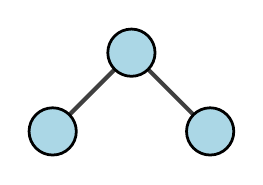
\begin{tikzpicture}
    %Nodes
    \Vertex[x=1,y=1]{A}
    \Vertex[x=0,y=0]{B}
    \Vertex[x=2,y=0]{C}
    %Edges
    \Edge(A)(B)
    \Edge(A)(C)
\end{tikzpicture}
\end{center}
While the above example is a simple network, this model can be further extended through:
\begin{itemize}
    \item Adding directions to edges (from one node to another)
    \item Adding weights to edges (often representing data about node interactions)
    \item Adding attributes to nodes themselves (binary,discrete or continuous)
\end{itemize}
An example of a directed, weighted biological network with low assortativity is a gene expression network (nodes:genes, edges:transcription level correlations) with few transcription factors which each modulates expression of multiple unrelated genes.
For this project, nodes will represent \ac{otu}s and edges will represent genetic exchange between those \ac{otu}s, whereas in normal phylogenies, edges only represent taxonomic relationships.
Despite the complexity of \ac{hgt}, network theory allows a flexible theoretic framework to analyze these interactions that are normally ignored by traditional phylogenetic methods.
\section*{Phylogenomic Networks}
\ac{hgt} is an important factor in understanding evolution in prokaryotes.
Since \ac{hgt} has been found to be frequent throughout the prokaryotic tree of life, this has lead many to re-evaluate the concept of a ``tree of life'', which by definition ignores these horizontal interactions\citep{netoflife}.
\subsection*{Prokaryotic Net Of Life}
In graph theory a tree is defined as a graph where there is only one path between every pair of nodes.
In phylogenetics this implies there is only one path for genetic material to transfer between organisms, that path being vertical inheritance.
As \ac{hgt} demonstrates, this tree model is clearly an incomplete representation of genetic relationships between \ac{otu}s.
Genetic material can be transferred outside of reproduction, allowing for multiple paths by which a single gene can be found in two \ac{otu}s (either inheritance, transfer or some combination of the two)\citep{lgt}.
This prompted the idea of a prokaryotic network of life (as opposed to a tree), with edges indicating both vertical and horizontal transfers of genetic material\citep{netoflife}.
Edges can now connect \ac{otu}s to closely or distantly related \ac{otu}s, and even extinct ancestral \ac{otu}s.
\subsection*{Detection}%cite with ihgt,hgterr
While understanding that \ac{hgt} is important and networks provide a useful theoretic framework to study it, constructing such networks is not trivial.
Many different strategies have been developed to detect potential \ac{hgt} events given a phylogenetic tree, with some able to detect both recipients and donors\citep{ihgt}.
There are two primary sets of methods for detecting \ac{hgt}.
\paragraph{Parametric}
These methods rely on investigating the sequence composition (GC\%, codon bias, etc.) in genes and when they deviate from the genomic average.
Average GC content has been found to vary significantly between some organisms, even by up to $30\%$ in closely related organisms\citep{ihgt}.
The same is true for codon bias, where codons variants are observed with different frequency in different bacteria, dependent on the expression levels of the tRNAs in those respective organisms\citep{ihgt,codonbias}.
For example, if \ac{ecoli} contains more copies of a tRNA with the anti-codon TTA (Leucine) than CTC, genes will more likely encode the TTA codon to increase transcription efficiency\citep{codonbias}.
If more TTA codons than CTC codons are observed in a gene in \ac{sau}, assuming \ac{sau} has no leucin codon bias, one may be able to infer that the codon-biased gene was transferred horizontally\citep{ihgt}.
Other metrics to consider are GC\%, k-mer frequency or the presence of other features around the candidate gene, such as transposases or flanking sequences\citep{ihgt}.
\paragraph{Phylogenetic}
These methods rely on recognizing discordance between gene trees and species trees.
If a gene tree is found to have a significantly different topology from a species tree, this difference may be the result of an \ac{hgt} event\citep{hgterr}.
One can also compare the substructures of a gene trees and species trees (created by removing a set of edges leaving a set of sub-trees) to see if the tree substructures disagree\citep{ihgt}.
Another strategy involves pruning (removing an edge to get 2 distinct trees) an internal branch and reattaching the subtrees at a different location.
If the re-grafted tree has a better fit to the reference tree than the original, this may be indicative of an \ac{hgt} event between the original node and the node the subtree was re-grafted to\citep{ihgt}.\par
While \ac{hgt}s can lead to these discordances, there are other series of evolutionary events than can produce the same results\citep{hgterr}.
Events that may lead to false diagnosis of \ac{hgt} are: incomplete lineage sorting, gene duplication followed by loss in one of the descendant lineages or homologous recombination\citep{ihgt,hgterr}.
Strategies to account for these events, as well as account uncertainty in the tress themselves exist, but there still exist other sources that remain unaccounted for\citep{hgterr}.\par
It should also be noted that many of these methods require heuristic solutions, as they are computationally expensive, and sometimes even entirely intractable, which creates further uncertainty in the results obtained\citep{ihgt}.
As an example, finding the minimum edit path between 2 trees (as in the re-grafting method) is NP-Hard, but the solution space can be limited by not considering pruning branches between consistent nodes\citep{sprnp,ihgt}.\par\par
Generally phylogenetic methods are preferred for multiple reasons:
\begin{itemize}
    \item Can make use of multiple genomes at once\citep{ihgt}
    \item Require explicit evolutionary models, which come with their own framework for hypothesis testing and model selection\citep{ihgt}.
    \item \ac{hgt} events identified by parametric methods are often found by phylogenetic methods as well\citep{ihgt}.
    \item In recent years, the requirements of computing power and  multiple well sequenced genomes for phylogenetic methods have become easier and easier to meet\citep{ihgt}.
\end{itemize}
While detecting \ac{hgt} events with high degrees of certainty is still difficult, much progress has been made in recent years,especially using phylogenetic methods\citep{ihgt}.
\section*{Do CRISPR Systems Affect Horizontal Gene Transfer?}
Yes.
\subsection*{Interference Mechanisms}
Since \ac{crsp}s have been shown to be capable of interfering with conjugation (conjugative plasmid specific spacers) and transduction (phage immunity), it has been hypothesized that lower rates of \ac{hgt} will be observed in strains with \ac{crspc} systems\citep{staphlim}.
\ac{crspc} systems have also been found to interfere with transformation-mediated \ac{hgt}, by degrading foreign DNA taken up by a cell\citep{climtrans}.
\subsection*{Complexities And Costs Of CRISPR-Cas Systems}
As noted above, \ac{crspc} systems have been shown to interfere with plasmid conjugation in \ac{sau} by integrating a spacer targeting the \textit{nickase} sequence, necessary for conjugation in \ac{sau}\citep{staphlim}.
Since antibiotic resistance genes are often transferred on plasmids, this can incur a significant cost, especially in environments with large amounts of antibiotics (ex: hospitals, trees etc.)\citep{hospital}.
\ac{crspc} systems incur a metabolic cost, as \ac{cas} proteins, guide RNAs, spacer acquisition proteins must all be expressed to maintain immunity\citep{crispgen}.
Despite primarily being an immune system, the way \ac{crspc} functions (degrading foreign DNA matching spacers motifs, resisting phage infection) can have off-target effects on \ac{hgt}\citep{acqorres}.
While resisting lytic phage infection clearly provides some fitness benefit, \ac{crspc} has also been shown to resist prophage incorporation\citep{acqorres}.
Prophages can serve as vectors for \ac{hgt}, but they can also provide super-infection immunity, and even reduce competitor bacterial populations through infection\citep{acqorres,transhgt}.
It has also been shown that spacer sequences representative of a bacterium's own chromosomal DNA can be incorporated in to \ac{crsp} array, leading to an auto-immune response where \ac{cas} proteins target native host DNA\citep{selfcrisp}.
As \ac{crspc} systems persist, anti-\ac{crsp} mechanisms have evolved in certain phages, making them immune to CRISPR-Cas, denoted anti-\ac{crsp}s\citep{acqorres}.
This has a two-fold effect, as it can increase the susceptibility of the host to infection, reducing the fitness benefit of CRISPR-Cas, but it can also allow for more transduction-mediated \ac{hgt}\citep{acqorres}.
\subsection*{Potential Strategies For Reducing CRISPR-\ac{hgt} Trade-off Costs}
Due to the  myriad of fitness costs associated with consistently expressing \ac{crspc} systems, bacteria have appeared to develop strategies to mitigate these costs.
While \ac{crspc} systems can confer a fitness advantage by providing immunity to phage infection, the fitness cost associated is complex, especially as \ac{crspc} systems  themselves can be transferred  horizontally, either on a plasmid or even through transduction\citep{crisprlgt}.
It has been posited that \ac{crspc} systems need only be present in a few members of a population at once and transferred between members to maintain phage immunity while reducing the cost of constantly maintaining \ac{crspc} systems\citep{acqorres}.
It has been found that the presence of a \ac{crsp} system does not necessarily imply activity of the system, creating new mechanism(s) by which the fitness cost of \ac{crspc} systems can be reduced\citep{acqorres}.
The presence of \ac{crspc} systems have also been shown to actually enhance \ac{hgt} via transduction at the population level by reducing total phage abundance\citep{transhgt}.
The presence of \ac{crspc} systems in Firmicutes have been shown to be associated with increased levels of gene insertion and deletion compared to closely related outgroups, further demonstrating the complexity of this relationship\citep{athena}.
The effects of \ac{crspc} systems on rates of \ac{hgt} are highly complex, owning in no small part to the broad range of \ac{crsp} effects, how \ac{crsp} activity can be modulated and the transfer of \ac{crsp} systems themselves within a population\citep{acqorres}.
Taking a systematic approach may help elucidate the dynamics between \ac{crsp} system presence and \ac{hgt} rate.
\section*{\huge Hypothesis}
The null hypothesis is that bacterial strains/genera with known \ac{crsp} systems will show no significant differences in network statistics to those strains/genera without known \ac{crsp} systems.
\section*{\huge Objectives}
Using sequenced genomes, the goal of this project is to construct phylogenetic networks for all strains within sets of genera with and without \ac{crspc} systems.
Ultimately the goal of this project is to examine the relationship of \ac{hgt} rates and the presence of \ac{crspc} systems, using a network theoretic approach. The following sets of comparisons will contribute to the understanding of this relationship:
\paragraph*{Within Network Comparisons}%2 sentences
For genera with strains containing \ac{crsp} and Non-\ac{crsp} species, comparing the network dynamics of those sets of nodes across genera will elucidate if \ac{crspc} systems affect the \ac{hgt} rates or the association patterns of individual \ac{otu}s.
\paragraph*{Between Network Comparisons}%2 sentences
Networks created from genera with no known \ac{crsp} system containing strains (nc-networks) will be compared to mixed networks, containing strains both with and without \ac{crsp} Systems.
This will help determine whether the presence of \ac{crsp} nodes can affect \ac{hgt} network dynamics of \ac{otu}s other than themselves.
A simple example may be that if mixed networks show more overall transfers across the network than nc-networks, \ac{crsp} containing \ac{otu}s may be increasing \ac{hgt} among closely related Non-\ac{crsp} \ac{otu}s.
\paragraph*{Gene Indel Rates Vs. Network Statistics}%2 sentences
Comparing insertion and  deletion rates independantly can help further specify what mechanisms may be responsible for trends observed in network statistics.
If a mixed network is found to be density connected, but also shows a deletion bias, this may imply that most of the genes being transferred may not confer a fitness advantage.
\section*{\huge Methods}
\subsection*{Summary}
The goal of the project is to create a phylogenetic network from a set of GenBank (.gbff) files, in this case all full genomes for a given bacterial genus, for analysis of \ac{hgt}.
The workflow is as follows:
\begin{enumerate}
    \item Download genomes
    \item Filter mobile genetic elements from genomes
    \item Cluster all genes into families using Diamond (\% identity > 80)
    \item Construct a presence/absence matrix of gene families
    \item Estimate gene insertion/deletion rates separately for the CRISPR and non-CRISPR containing genomes using the package markophylo (4 rates total)
    \item Construct a species tree using all gene families that have only 1 member (gene) in each genome
    \begin{enumerate}
        \item Create a sequence alignment for each gene family
        \item Concatenate all alignments together
        \item Build tree using Mr Bayes (10000 generations, 25\% burn in)
    \end{enumerate}
    \item Construct a gene tree for each gene family
    \begin{enumerate}
        \item Only consider families with a gene belonging in at least 30\% of the genomes analyzed (ex: a family with 6 genes in 4 of 15 genomes)
        \item Align each family
        \item Build tree using Mr Bayes (10000 generations, 25\% burn in)
    \end{enumerate}
    \item Use the program HiDe to infer a phylogenetic network from the species tree and gene trees.
    \item Annotate the network with CRISPR data scraped from the CRISPR-one database.
    \item Using the gene insertion/deletion estimated and the annotated networks see if there is any significant difference in the dynamics of \ac{hgt} between organisms with CRISPR and without CRISPR systems.
\end{enumerate}
\subsection*{Data Collection}
Complete genomes from NCBI RefSeq are downloaded and the \ac{crsp}db (along with a python script) is used to annotate genera as being mixed (containing strains with and without \ac{crspc} systems) or Non-\ac{crsp} (containing no strains with a \ac{crspc} system)\citep{crispdb}.
\ac{crsp} annotations of \ac{cas}, Cfp proteins from NCBI and the \ac{crsp}one tool from Zhang and Ye will also be used to assess the presence of \ac{crsp} systems\citep{ineqcas}.
\subsection*{Gene Presence/Absence Matrix}
In order to use the program markophylo to estimate insertion and deletion rates, a \ac{pa} matrix and a phylogenetic species tree are required.
First any genes classified as \ac{mge}s (from NCBI annotations) are removed.
Next genes are grouped into families by reciprocal BLAST hits and single link clustering.
The remaining unclassified genes are compared to the NCBI non-redundant database with BLAST to check if they are genes, and if they are then they are considered their own family with one member.
The \ac{pa} matrix is constructed as follows, for each \ac{otu} a binary vector is created, where each entry represents a gene family and a 1 indicates that that \ac{otu} contains 1 gene in that family.
This is repeated for all \ac{otu}s, creating a $G \times O$ binary matrix, where $G$ is the total number of gene families and $O$ is the number \ac{otu}s.\par
There are many ways to construct a species tree, but for this project the tree will be constructed using genes from gene families present in all \ac{otu}s being considered, using Bayesian methods, as implemented in the program MrBayes.
\subsection*{Makophylo Rate Estimations}
Given a species tree and a gene family \ac{pa} matrix for the \ac{otu}s of the species tree the R package \textit{markophylo} can provide gene insertion and gene deletion rate estimates\citep{marko}.
The presence or absence of gene families are considered 2 discrete states, for which a $(2\times 2)$ transition rate matrix (of a \ac{mc} model) can be estimated using maximum likelihood techniques.
The values in this estimated transition matrix are the insertion rate (transition probability of gene absence $\to$ presence) and deletion rate (transition probability of gene presence $\to$ absence)\citep{marko}.
\subsection*{Network Construction}
Quartet decomposition is method by which \ac{hgt} events can be identified using a set of gene trees and a species tree.
Given a tree $T$ a quartet is a subtree contain 4 of the leaf nodes in $T$, meaning that for a tree with $N$ leaf nodes (or \ac{otu}s) there are $\binom{N}{4}$ unique quartets in that tree.
A quartet $Q$ is considered consistent with a tree if $Q = T|Le(Q)$ where $T|Le(Q)$ is the tree obtained by suppressing all degree-two nodes in $T[X]$ and $T[X]$ is the minimal subtree of T with all nodes in $X$, which is a leaf set of $T$\citep{hide}.
To calculate the weight of an edge for the network, given a species tree $S$ and a set of gene trees $G$\citep{hide}:
\begin{enumerate}
    \item Pick a horizontal edge $H = ((u,v),(v,u))$ from $S$
    \item Pick a gene tree $G_i$ in $G$
    \item Decompose $G_i$ into it's set of quartets $\phi_i$
    \item Remove all quartets consistent with $S$ or previously explained from $\phi_i$
    \item Set $RS((u,v),\phi_i)$ to be the number of quartets in $\phi_i$ that support the edge $(u,v)$
    \item Set $NS((u,v),\phi_i)$ to be $RS((u,v),\phi_i)$ divided by $\lambda$, which is the total number of quartets in $S$ that are consistent with the edge $(u,v)$.
    \item The score for the edge $H$ for tree $G_i$ is $max\{NS((u,v),\phi_i),NS((v,u),\phi_i)\}$
    \item The total score for the edge $H$ is the sum of scores for each tree $G_i$
    \item This total score calculation is repeated for each horizontal edge $H_i$ in S, resulting in a list of edges, which is a complete description of the network.
\end{enumerate}
\subsection*{Network Statistics}
All networks will be comprised of nodes representing \ac{otu}s and weighted edges represent the estimated amount of \ac{hgt} events between the two incident nodes.
As multiple sets of networks can be computed for a single set of genera (using different sets of gene trees), bootstrap support for edges and confidence intervals on edge weights can also be calculated.
Given a network, with a set of nodes $V = \{V_0$ \dots $V_i\}$ of cardinality $N$ and a set of weighted edges (an unordered 2-tuple and weight) $T = \{((V_1,V_2),W_{1,2})$ \dots $((V_i,V_j),W_{i,j})\}$ with cardinality $E$ descriptive statistics can be computed as follows\citep{netstat}:
\begin{itemize}
    \item Total edge weight: sum of all edge weights in a network
    \item Average edge weight: sum of all edge weights divided by $N$
    \item Node Closeness Centrality:$ \frac{N-1}{\sum_v d(x,v)}$ where $d(x,y)$ is the length of the shortest path between node v and x.
    \item Node Associativity:$ \frac{j(j+1)(\overline{k}-\mu_q)}{2E\sigma^2_q}$ where $j$ is the excess degree of the node and $\overline{k}$ is the average excess degree of the node's neighbors and $\mu_q$ and $\sigma_q$ are the mean and standard variation of the excess degree distribution.
    \item Network Density:$ \frac{2(E-N+1)}{N(N-3)+2}$
    \item Node Clustering Coefficient:$ \frac{2e}{k(k-1)}$ where $k$ is the number of neighbors and $e$ is the number of edges between all neighbors.
    \item Network Diameter: The shortest path between the 2 furthest nodes in a network.
\end{itemize}
\section*{\huge Results \& Discussion}
Most of the pipeline is complete, however several things still need to be finished:
\begin{enumerate}
    \item Resolve errors in picking candidate genes for the species tree
    \item Resolve issues related to scaling up processes for large bacthes of input files
    \item Incorporate the results of markophylo into the analysis
    \item Decide on a sampling methodology for gene trees for building the phylogenetic networks
\end{enumerate}
Two networks were produced for the genera \textit{Ehrlichia} and \textit{Dehalococcoides}, using all available gene trees and the species tree for each.
\textit{Ehrlichia} contains 15 fully sequenced genomes, none of which have both Cas proteins and CRISPR arrays according to CRISPR-one.
%include figure
\begin{figure}[htb!]
    \makebox[\textwidth][c]{\includegraphics[width=0.8\linewidth]{../images/ehrlichia_network.png}}
    \caption{Phylogenetic network of all strains in the genus \textit{Ehrlichia}. Blue nodes indicate no CRISPR systems. Edge thickness is proportional to the number of gene transfers estimated between strains (thicker means more transfers)}
\end{figure}
\FloatBarrier
\textit{Dehalococcoides} contains 15 fully sequenced genomes 4 of which have both Cas proteins and CRISPR arrays according to CRISPR-one.
%include figure
\begin{figure}[htb!]
    \makebox[\textwidth][c]{\includegraphics[width=0.8\linewidth]{../images/dehalodeicoccus_network.png}}
    \caption{Phylogenetic network of all strains in the genus \textit{Dehalodeicoccus}. Blue nodes indicate no CRISPR systems. Edge thickness is proportional to the number of gene transfers estimated between strains (thicker means more transfers)}
\end{figure}
\FloatBarrier
From looking at these diagrams there appears to be more thick (i.e. high transfer rate) edges for \textit{Ehrlichia} than \textit{Dehalococcoides}, but the rest of the edges in \textit{Ehrlichia} are fairly thin as compared to \textit{Dehalococcoides}.
These networks do appear to be different in how they are organized, but why this is is not obvious and may be more related to the differences between these genera not related to the presence of \ac{crspc} systems.
%stats table
\begin{center}
    \begin{tabular}{l|r r}
        Metric & Ehrlichia & Dehalococcoides\\
        \hline
        Density & 0.952380952381&0.961904761905\\
        Average Edge Weight & 0.0748552512271&0.0695005449268\\
        Average Node Clustering Coefficient & 0.956&0.96\\
        Average Node Closeness Centrality & 0.9555555555555556&0.9644444444444444\\
        Average Node Communicability Betweenness Centrality & 0.5851751888088753 &0.5893446744946671\\
        Average Node Connectivity & 13.0952380952 & 13.2\\
    \end{tabular}
\end{center}
From this cursory overview of the statistics computed for these two genera, there appears to be no significant difference between  the two networks in terms of how the edges are connected or weighted, in line with the null hypothesis.
A much more rigorous statistical analysis of a much larger set of networks still remains to be conducted before any conclusions about \ac{hgt} or \ac{crspc} systems can be drawn.
The extent of this analysis is not nearly sufficient for inferring anything but demonstrates a proof of concept for this strategy of analysis.
\section*{\huge Significance \& Future Work}
The results of this work will hopefully shed light on how \ac{crspc} systems affect the rate of \ac{hgt}.
This can help identify new potential strategies for combating the spread of antibiotic resistance.
This study may also shed light on the fitness effects of \ac{crspc} systems and how they manifest at a population level.\par
There are multiple ways to expand this analysis to answer other questions related to the transfer of genes.
As \ac{hgt} inference methods improve and it becomes possible to discern the direction of transfer with confidence, a whole new set of techniques become available for study.
If one is interested in studying the transfer patterns of a specific grouping of genes, either by function, common structural motifs, sequence composition, expression pattern this type of analysis is highly suitable.
For example, the transfer of CRISPR systems themselves is something largely unstudied.
Networks can be constructed from Cas and Cfp1 genes as well as identified \ac{crsp} arrays to estimate how often \ac{crspc} systems themselves move around communities.
Networks constructed from ribosomal genes can be used as a reference point for what very little transfer looks like.
This pipeline provides a simple way to analyze trends \ac{hgt} between a set of specified organisms.
\printbibliography
\end{document}
